% TeX file "appendix"

% Research Module in Econometrics & Statistics 
% Prof. Dr. Liebl & Dr. Christopher Walsh
% Winter 2021/22, M.Sc. Economics, Bonn University
% Xingyu Tao, Xuan Li, Sven Jacobs


\phantomsection 
\addcontentsline{toc}{section}{Appendix} 

\section*{Appendix}

\subsection*{Appendix 1: Proofs} \label{appendix_1}

\begin{proof}[Proof (Theorem \ref{theorem_1})]
	Fix some $x$ in the interior of $\supp(f)$.
	We write
	\begin{align}
		Y_i &= m(X_i) + \epsilon_i \\
		    &= m(x) + [m(X_i) - m(x)] + \epsilon_i \,.
	\end{align}
	It then also holds that
	\begin{align}
		\frac{1}{nh} \sum_{i = 1}^{n} K \left( \frac{X_i - x}{h} \right) Y_i &=
		\frac{1}{nh} \sum_{i = 1}^{n} K \left( \frac{X_i - x}{h} \right) m(x) \\
		&+ \underbrace{\frac{1}{nh} \sum_{i = 1}^{n} K \left( \frac{X_i - x}{h} \right) [m(X_i) - m(x)]}_{\equiv \, \hat{g}_1(x)} +
		\underbrace{\frac{1}{nh} \sum_{i = 1}^{n} K \left( \frac{X_i - x}{h} \right) \epsilon_i}_{\equiv \, \hat{g}_2(x)} \,.  
	\end{align}
	Dividing by the standard kernel density estimator $\hat{f}(x)$ yields
	\begin{equation}
		\hat{m}_{\NW}(x) = m(x) + \frac{\hat{g}_1(x)}{\hat{f}(x)} + \frac{\hat{g}_2(x)}{\hat{f}(x)} \,. \label{eq:appendix_1_01}
	\end{equation}
	
	We first derive $\E[\hat{m}_{\NW}(x) \,|\, \bm{X}]$.
	Since $\E[\epsilon_i \,|\, X_i] = 0$, we immediately get $\E[\hat{g}_2(x) \,|\, \bm{X}] = 0$.
	For $\hat{g}_1(x)$ we have
	\begin{equation}
		\E[\hat{g}_1(x) \,|\, \bm{X}] = \frac{1}{h} \E \left[ K \left( \frac{X - x}{h}  \right) [m(X) - m(x)] \right] \,.
	\end{equation}
	Writing the expectation as an integral with respect to the design density $f$ and applying variable substitution leads to
	\begin{align}
		\E[\hat{g}_1(x) \,|\, \bm{X}] &= \int_{-\infty}^{\infty} \frac{1}{h} K \left( \frac{z - x}{h} \right) [m(z) - m(x)] f(z) \diff z \\
		&= \int_{-\infty}^{\infty} K(u) [m(x + hu) - m(x)] f(x + hu) \diff u \,. \label{eq:appendix_1_02}
	\end{align}
	In the next step we write $m(x + hu)$ and $f(x + hu)$ as Taylor expansions around $x$:
	\begin{align}
		m(x + hu) &= m(x) + m'(x)hu + \frac{1}{2} m''(x)h^2u^2 + \littleO(h^2) \,, \\
		f(x + hu) &= f(x) + f'(x)hu + \littleO(h) \,.
	\end{align} 
	Plugged into \eqref{eq:appendix_1_02} we obtain
	\begin{align}
		\E[\hat{g}_1(x) \,|\, \bm{X}] &= \int_{-\infty}^{\infty} K(u) \left[ m'(x)hu + \frac{1}{2} m''(x)h^2u^2 + \littleO(h^2) \right] [f(x) + f'(x)hu + \littleO(h)] \diff u \label{eq:appendix_1_03} \\ 
		&= h \int_{-\infty}^{\infty} uK(u) \diff u \, m'(x) [f(x) + \littleO(h)] \label{eq:appendix_1_04} \\
		&+ h^2 \int_{-\infty}^{\infty} u^2K(u) \diff u \left[ \frac{1}{2} m''(x) f(x) + m'(x) f'(x) \right] \\
		&+ h^3 \int_{-\infty}^{\infty} u^3K(u) \diff u \, \frac{1}{2} m''(x) f'(x) \\
		&+ \littleO(h^2) \,.
	\end{align}
	Due to the symmetry of the kernel from Assumption \ref{A4} odd kernel moments vanish. Hence, we can write with the definition of $\kappa_2(K)$ 
	\begin{equation}
		\E[\hat{g}_1(x) \,|\, \bm{X}] = \frac{1}{2} \kappa_2(K) m''(x) h^2 f(x) + \kappa_2(K) m'(x)f'(x) h^2 + \littleO(h^2) \,.
	\end{equation}
	With \eqref{eq:appendix_1_01} and the consistency of the kernel density estimator \parencite{Parzen_1962}, i.e.\ $\hat{f}(x) \overset{p}{\longrightarrow} f(x)$,
	we arrive at the desired expression
	\begin{equation}
		\ABias (\hat{m}_{\NW}(x) \,|\, \bm{X}) = \frac{1}{2} \kappa_2(K) m''(x) h^2 + \kappa_2(K) \frac{m'(x)f'(x)}{f(x)} h^2 \,.	
	\end{equation}

	We now derive $\Var(\hat{m}_{\NW}(x) \,|\, \bm{X})$.
	For $\hat{g}_2(x)$ we get
	\begin{align}
		\Var(\hat{g}_2(x)) &= \frac{1}{nh^2} \E \left[ K \left( \frac{X_i - x}{h} \right) \epsilon_i \right]^2 \,, \\
		\Var(\hat{g}_2(x) \,|\, \bm{X}) &= \frac{1}{nh^2} \E \left[ K \left( \frac{X_i - x}{h} \right)^2 \sigma^2(X_i) \right] \,.
	\end{align}
	Writing the expectation as an integral with respect to the design density $f$ and applying variable substitution leads to
	\begin{align}
		\Var(\hat{g}_2(x) \,|\, \bm{X}) &= \frac{1}{nh^2} \int_{-\infty}^{\infty} K \left( \frac{z - x}{h} \right)^2 \sigma^2(z) f(z) \diff z \\
		&= \frac{1}{nh} \int_{-\infty}^{\infty} K(u)^2 \sigma^2(x + hu) f(x + hu) \diff u \,.
	\end{align}
	Writing $\sigma^2(x + hu)$ and $f(x + hu)$ as first-order Taylor expansions around $x$ and using the definition of $R(K)$ we arrive at
	\begin{equation}
		\Var(\hat{g}_2(x) \,|\, \bm{X}) = R(K) \sigma^2(x) f(x) \frac{1}{nh} + \littleO \left( \frac{1}{nh} \right) \,.
	\end{equation}
	For $\hat{g}_1(x)$ a similar expansion as was done for its expectation yields $\Var(\hat{g}_1(x) \,|\, \bm{X}) \sim \frac{h^2}{nh}$ which is of smaller order than $(nh)^{-1}$.
	With \eqref{eq:appendix_1_01} and $\hat{f}(x) \overset{p}{\longrightarrow} f(x)$ we obtain the desired expression
	\begin{equation}
		\AVar (\hat{m}_{\NW}(x) \,|\, \bm{X}) = \frac{R(K) \sigma^2(x)}{f(x)} \frac{1}{nh} \,.
	\end{equation} 
\end{proof}

\begin{proof}[Proof (Theorem \ref{theorem_4})]
	In Section \ref{subsec:definition} we have seen that
	\begin{equation}
		\hat{m}_{\LL}(x) = \bm{e}_1^\top \left( \bm{X}_x^\top \bm{W}_x^{\vphantom{\top}} \bm{X}_x^{\vphantom{\top}} \right)^{-1} \bm{X}_x^\top \bm{W}_x^{\vphantom{\top}} \bm{Y} \,.
	\end{equation}
	The general solution of the local polynomial estimator of degree $p$ can be computed as (e.g.\ \cite{Hastie_1993})
	\begin{align}
		\hat{m}_{\LP}(x; p) &= \bm{b}_x^\top \left( \bm{\tilde{X}}_x^\top \bm{W}_x^{\vphantom{\top}} \bm{\tilde{X}}_x^{\vphantom{\top}} \right)^{-1} \bm{\tilde{X}}_x^\top \bm{W}_x^{\vphantom{\top}} \bm{Y} \\
							&= \sum_{i = 1}^{n} w_i(x) Y_i \,,
	\end{align}
	where invertibility of $\bm{\tilde{X}}_x^\top \bm{W}_x^{\vphantom{\top}} \bm{\tilde{X}}_x^{\vphantom{\top}}$ is assumed and
	\begin{equation}
		\bm{Y} = \begin{bmatrix} Y_1 \\ \vdots \\ Y_n \end{bmatrix},
		\bm{\tilde{X}}_x = \begin{bmatrix} 1 & X_1 & \dots & X_1^p \\ \vdots & \vdots & \ddots & \vdots \\ 1 & X_n & \dots & X_n^p \end{bmatrix},
		\bm{W}_x = \diag \left\{ K \left( \frac{X_1 - x}{h} \right), \dots, K \left( \frac{X_n - x}{h} \right) \right\},
		\bm{b}_x = \begin{bmatrix} 1 \\ x \\ \vdots \\ x^p \end{bmatrix} \,.
	\end{equation}
	With $\bm{v}_j^\top \equiv (X_1^j, X_2^j, \dots, X_n^j)$ for $j = 0, 1, \dots, p$ we can write
	\begin{equation} \label{eq:appendix_1_05}
		\bm{b}_x^\top \left( \bm{\tilde{X}}_x^\top \bm{W}_x^{\vphantom{\top}} \bm{\tilde{X}}_x^{\vphantom{\top}} \right)^{-1} \bm{\tilde{X}}_x^\top \bm{W}_x^{\vphantom{\top}} \bm{v}_j = \sum_{i = 1}^{n} w_i(x) X_i^j \,.
	\end{equation}
	Applying \eqref{eq:appendix_1_05} for each $j = 0, 1, \dots, p$ and noticing that $\bm{\tilde{X}}_x = [\bm{v}_0, \bm{v}_1, \dots, \bm{v}_p]$ gives for the LHS of \eqref{eq:appendix_1_05}
	\begin{align}
		&\bm{b}_x^\top \left( \bm{\tilde{X}}_x^\top \bm{W}_x^{\vphantom{\top}} \bm{\tilde{X}}_x^{\vphantom{\top}} \right)^{-1} \bm{\tilde{X}}_x^\top \bm{W}_x^{\vphantom{\top}} \bm{\tilde{X}}_x^{\vphantom{\top}} \\
		= \,\, &\bm{b}_x^\top \\
		= \,\, &[1, x, \dots, x^p]
	\end{align}
	and for the RHS
	\begin{equation}
		\left[ \sum_{i = 1}^{n} w_i(x), \sum_{i = 1}^{n} w_i(x) X_i, \dots, \sum_{i = 1}^{n} w_i(x) X_i^p \right] \,.
	\end{equation}
	By component matching we obtain
	\begin{equation}
		x^j = \sum_{i = 1}^{n} w_i(x) X_i^j \,,
	\end{equation}
	such that for $j = 0$ and $j = 1$:
	\begin{align}
		1 &= \sum_{i = 1}^{n} w_i(x) \,, \\
		x &= \sum_{i = 1}^{n} w_i(x) X_i \,.
	\end{align}
	If we combine these two equations (multiplying the first by $x$) we arrive at the desired result
	\begin{equation}
		\sum_{i = 1}^{n} w_i(x) (X_i - x) = 0 \,.
	\end{equation} 
\end{proof}

\newpage

\subsection*{Appendix 2: Kernels} \label{appendix_2}

The following is a short excursus on the optimal kernel choice.
When calculating the minimal asymptotic error functions $\AMSE_{\text{opt}}$ and $\AMISE_{\text{opt}}$ following Section~\ref{subsec:theoretical_comparison}, the dependence on the kernel can be seen to be $R(K)^{4/5} \kappa_2(K)^{2/5}$.
This dependence is the same for kernel density estimation \parencite[49]{Müller_1988}.
The kernel minimizing the expression is the Epanechnikov kernel $K_\text{E}(u) = \frac{3}{4}(1 - u^2)$ as was proved first by \textcite{Epanechnikov_1969} in the context of density estimation.
The efficiency of a kernel is then defined relative to the optimal Epanechnikov kernel by 
\begin{equation}
	\Eff(K) \equiv \frac{R(K_{\text{E}}) \kappa_2(K_{\text{E}})^{1/2}}{R(K) \kappa_2(K)^{1/2}} \,.
\end{equation}
Table~\ref{tab:kernels} lists the efficiency scores for kernels mostly applied in practice.
\textcite[Section~5]{Müller_1988} provides a thorough treatment of optimal kernel theory including, for instance, optimal higher-order kernel functions.
\vfill
\renewcommand{\arraystretch}{1.4}	
\begin{table}[h]
	\centering
	\captionabove{Prominent kernels with their constants and efficiency}
	\label{tab:kernels}
	\begin{tabular}{l l c c c c}  
		\toprule
		Kernel & Function & Support & $R(K)$ & $\kappa_2(K)$ & Efficiency \\
		\midrule
		Epanechnikov & $K_\text{E}(u) = \frac{3}{4}(1 - u^2)$                     & $[-1, 1]$    & $\frac{3}{5}$           & $\frac{1}{5}$ & 100.0\% \\
		Biweight     & $K_\text{B}(u) = \frac{15}{16}{(1 - u^2)}^2$               & $[-1, 1]$    & $\frac{5}{7}$           & $\frac{1}{7}$ & 99.39\% \\
		Triangular   & $K_\text{T}(u) = 1 - |u|$                                  & $[-1, 1]$    & $\frac{2}{3}$           & $\frac{1}{6}$ & 98.59\% \\
		Gaussian     & $K_\text{G}(u) = \frac{1}{\sqrt{2\pi}}\e^{-\frac{u^2}{2}}$ & $\mathbb{R}$ & $\frac{1}{2\sqrt{\pi}}$ & $1$           & 95.12\% \\
		Uniform      & $K_\text{U}(u) = \frac{1}{2}$                              & $[-1, 1]$    & $\frac{1}{2}$           & $\frac{1}{3}$ & 92.95\% \\
		\bottomrule
	\end{tabular}	
\end{table}
\renewcommand{\arraystretch}{1.0}
\vfill
\begin{figure}[h]
	\centering	
	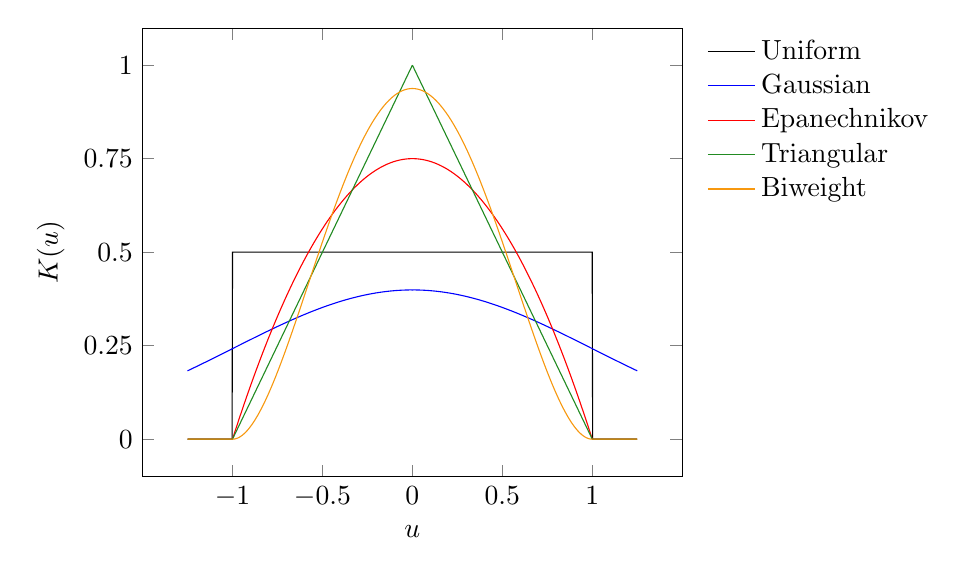
\begin{tikzpicture}
		\begin{axis}
			[
			grid, grid style={white}, 
			samples=1000, 
			domain=-1.25:1.25, 
			xlabel=$u$, xtick={-1, -0.5, 0, 0.5, 1},
			ylabel=$K(u)$, ytick={0, 0.25, 0.5, 0.75, 1},
			legend entries={Uniform, Gaussian, Epanechnikov, Triangular, Biweight},
			legend pos=outer north east,
			legend style={draw=none}, legend cell align={left}
			]
			
			\addplot[black]
			expression {1/2 * (abs(x)<1)};
			
			\addplot[blue]
			expression {1/(sqrt(2*pi)) * exp(-1/2*x^2)};
			
			\addplot[red]
			expression {3/4 * (1 - x^2) * (abs(x)<1)};
			
			\addplot[ForestGreen]
			expression {(1 - abs(x)) * (abs(x)<1)};
			
			\addplot[YellowOrange]
			expression {15/16 * (1 - x^2)^2 * (abs(x)<1)};
		\end{axis}
	\end{tikzpicture}
	\caption{Prominent kernels as given in Table~\ref{tab:kernels}}
\end{figure}

\newpage

\subsection*{Appendix 3: Additional material -- Theoretical description}
\vfill
\begin{figure}[h]
	\centering
	\includegraphics[trim=20 15 20 50, clip, width=0.75\textwidth]{figure_08.pdf}
	\caption{Nadaraya-Watson estimator in the case of linear regression, $m(x) = -1 + 2x$.
			 The realizations of $X$ are drawn from a uniform distribution and for clarification no noise is added.
		 	 The boundary effects are clearly visible, namely the bending of the straight line to a constant at the edges.}
	\label{fig:boundary_effects_linear}
\end{figure}
\vfill
\begin{figure}[h]
	\centering
	\includegraphics[trim=20 15 20 50, clip, width=0.75\textwidth]{figure_09.pdf}
	\caption{Local linear estimator compared to the Nadaraya-Watson estimator for 100 simulated observations}
	\label{fig:ll}
\end{figure}
\vfill
\begin{figure}
	\centering
	\includegraphics[trim=20 15 20 50, clip, width=0.75\textwidth]{figure_10.pdf}
	\caption{Boundary-adjusted Nadaraya-Watson estimator compared to the standard Nadaraya-Watson estimator and the local linear estimator for 100 simulated observations.
			 For explicit boundary adjustment the Epanechnikov boundary kernel from Section~\ref{sec:boundary_kernels} is used.}
	\label{fig:nw_boundary_adjusted}
\end{figure}

\begin{figure}
	\centering
	\includegraphics[trim=20 0 20 45, clip, width=0.75\textwidth]{figure_11.pdf}
	\caption{Effective kernel for the boundary-adjusted Nadaraya-Watson estimator and the local linear estimator when estimating at the lower boundary $x = 0$.
			 The effective kernel is given by the filled squares.}
	\label{fig:effective_kernel_nw_boundary}
\end{figure}

\clearpage

\subsection*{Appendix 4: Additional material -- Simulation}
\vfill
\begin{figure}[h!]
	\centering
	\begin{subfigure}{\textwidth}
		\centering
		\begin{tikzpicture}
			\begin{axis}
				[
				grid, grid style={white}, 
				samples=1000, 
				domain=0:1
				]
			
				\addplot[black]
				expression {sin(deg(2*pi*x))};
			\end{axis}
		\end{tikzpicture}
		\caption{$m_1(x) = \sin(2 \pi x)$ on the interval $[0, 1]$}
		\label{fig:m_1}
	\end{subfigure}
	\\[2ex]
	\begin{subfigure}{\textwidth}
		\centering
		\begin{tikzpicture}
			\begin{axis}
				[
				grid, grid style={white}, 
				samples=1000, 
				domain=0:1
				]
		
				\addplot[black]
				expression {2 - 2*x + 2*exp(-(x - 0.5)^2 / 0.01)};
			\end{axis}
		\end{tikzpicture}
		\caption{$m_2(x) = 2 - 2x + 2\exp \{ - (x - 0.5)^2 / 0.01 \} $ on the interval $[0, 1]$}
		\label{fig:m_2}
	\end{subfigure}
	\\[2ex]
	\begin{subfigure}{\textwidth}
		\centering
		\begin{tikzpicture}
			\begin{axis}
				[
				grid, grid style={white}, 
				samples=1000, 
				domain=0:1
				]
		
				\addplot[black]
				expression {2 - 2*x + 2*exp(-(x - 0)^2 / 0.01)};
			\end{axis}
		\end{tikzpicture}
		\caption{$m_3(x) = 2 - 2x + 2\exp \{ - (x - 0)^2 / 0.01 \} $ on the interval $[0, 1]$}
		\label{fig:m_3}
	\end{subfigure}
	\caption{Regression functions chosen for the simulation study}
	\label{fig:simulation_functions}
\end{figure}
\vfill
\begin{figure}
	\centering
	\begin{tikzpicture}
		\begin{axis}
			[
			grid, grid style={white}, 
			samples=1000, 
			domain=-0.25:1.25
			]
			
			\addplot[black]
			expression {3*(5/12 - (x - 0.5)^2) * (x>0) * (x<1)};
		\end{axis}
	\end{tikzpicture}
	\caption{Clustered design density $f_{\ast}$}
	\label{fig:clustered_design_density}
\end{figure}

\begin{figure}
	\centering
	\includegraphics[trim=20 15 20 50, clip, width=0.75\textwidth]{figure_14.pdf}
	\caption{Nadaraya-Watson fit and the regression function $m_1$ over the left boundary region (yellow-shaded),
			 for a random sample of $n = 100$ observations.
			 The dark yellow area reflects the integrated error.}
	\label{fig:simulation_set-up}
\end{figure}

\clearpage

\subsection*{Appendix 5: Additional material -- Application}
\vfill
\begin{figure}[h]
	\centering
	\includegraphics[trim=0 15 20 50, clip, width=0.75\textwidth]{figure_15.pdf}
	\caption{Democrats' probability of victory in election $t+1$, by margin of victory in election $t$.
			 Local averages are given by the filled circles.}
	\label{fig:application_overview}
\end{figure}
\vfill
\begin{figure}
	\centering
	\begin{subfigure}{0.75\textwidth}
		\centering
		\includegraphics[trim=0 0 20 45, clip, width=\textwidth]{figure_16a.pdf}
		\caption{Nadaraya-Watson estimator}
		\label{fig:application_left_nw}
	\end{subfigure}

	\begin{subfigure}{0.75\textwidth}
		\centering
		\includegraphics[trim=0 0 20 40, clip, width=\textwidth]{figure_16b.pdf}
		\caption{Local linear estimator}
		\label{fig:application_left_ll}
	\end{subfigure}
	\caption{CV error over a grid of 200 bandwidths for the left side to the threshold in Figure~\ref{fig:application_fits}.
			 The optimal bandwidth is indicated by the red line.}
	\label{fig:application_left}
\end{figure}

\begin{figure}
	\centering
	\begin{subfigure}{0.75\textwidth}
		\centering
		\includegraphics[trim=0 0 20 45, clip, width=\textwidth]{figure_17a.pdf}
		\caption{Nadaraya-Watson estimator}
		\label{fig:application_right_nw}
	\end{subfigure}
	
	\begin{subfigure}{0.75\textwidth}
		\centering
		\includegraphics[trim=0 0 20 45, clip, width=\textwidth]{figure_17b.pdf}
		\caption{Local linear estimator}
		\label{fig:application_right_ll}
	\end{subfigure}
	\caption{CV error over a grid of 200 bandwidths for the right side to the threshold in Figure~\ref{fig:application_fits}.
			 The optimal bandwidth is indicated by the red line.}
	\label{fig:application_right}
\end{figure}